\documentclass[%
  reprint,
  showpacs,
  showkeys,
  prl,
  floatfix
]{revtex4-2}

\usepackage[utf8]{inputenc}
\usepackage[T1]{fontenc}
\usepackage{amsmath,amssymb,amsfonts}
\usepackage{graphicx}
\usepackage{bm}
\usepackage[colorlinks=true,linkcolor=blue,citecolor=blue,urlcolor=blue]{hyperref}
\usepackage{microtype}
\usepackage{orcidlink}
\usepackage{pgfplots}
\pgfplotsset{compat=1.17}

\begin{document}

\title{All Correlations Yield the Same Peak Work, But Quantum is a Better Fuel}

\author{Karl Svozil\,\orcidlink{0000-0001-6554-2802}}
\email{karl.svozil@tuwien.ac.at}
\homepage{http://tph.tuwien.ac.at/~svozil}
\affiliation{Institute for Theoretical Physics, TU Wien, Wiedner Hauptstrasse 8-10/136, 1040 Vienna, Austria}

\date{\today}

\begin{abstract}
Initial system-environment correlations are a thermodynamic resource, enabling work extraction via their erasure. We compare the work potential of classical, quantum, and hypothetical stronger-than-quantum correlations as a function of measurement misalignment. While all models can yield a peak extractable work of $k_B T \ln 2$, corresponding to a mutual information of $\ln 2$, their value as a resource differs critically in its robustness. The classical resource is fragile, decaying linearly with misalignment, whereas the quantum resource is robust, decaying only quadratically. This hierarchy in operational robustness is quantitatively expressed in a thermodynamic version of the CHSH inequality based on extractable work.
\end{abstract}

\maketitle

\textit{Introduction}.---Classical thermodynamics defines an isolated system by boundaries impermeable to matter and energy. This picture is challenged by microscopic systems prepared with initial correlations to their environment. Even when sealed against energy exchange, such a system's local state can be altered by operations on its correlated environmental counterpart. An agent possessing side information can consume these correlations to perform work, a process governed by generalized thermodynamic laws that incorporate information-theoretic balances~\cite{Bera2017a,delrio2011thermodynamic,Sagawa2012}.

This Letter demonstrates that the nonlocal character of a correlation law maps directly to its operational value as a thermodynamic resource. We show that while classical, quantum, and stronger-than-quantum correlations share the same peak energetic value, they exhibit a clear hierarchy in their robustness against experimental imperfection.

The foundation of this analysis is the generalized second law for a system A interacting with a thermal bath E at temperature $T$. For a cyclic process on A (where its free energy change $\Delta F_T(\rho_A)=0$) that begins with mutual information $I_i(A:E)$ and ends in an uncorrelated state, the bound on extractable work is~\cite[Equ.~(4)]{Bera2017a}:
\begin{equation}
W_{\mathrm{ext}} \le k_{\mathrm{B}} T\, I_i(A:E).
\label{eq:work_from_I}
\end{equation}
This central result recasts mutual information as a thermodynamic fuel. It also refines the concept of isolation: a system is truly isolated only if it is both energetically sealed and initially uncorrelated with its surroundings.

\textit{A Hierarchy of Correlation Laws}.---We analyze three bipartite correlation laws $E(\theta)$ for $\{\pm1\}$-outcome measurements as a function of the relative angle $\theta \in [0, \pi]$ between settings. Their nonlocality is gauged by the Clauser-Horne-Shimony-Holt (CHSH) parameter $\mathcal{S}_{\mathrm{CHSH}}$, for which local realism imposes a bound of 2, quantum mechanics a bound of $2\sqrt{2}$~\cite{cirelson:80}, and the no-signaling principle an algebraic limit of 4. The three models are (see Fig.~\ref{fig:correlations}):
\begin{enumerate}
    \item \textbf{Classical (linear):} $E_c(\theta) = -1 + 2\theta/\pi$. This model arises from local hidden variables and saturates the classical bound, $\mathcal{S}_{\mathrm{CHSH}}^{(c)} = 2$.
    \item \textbf{Quantum (cosine):} $E_q(\theta) = -\cos\theta$. This describes measurements on a two-qubit singlet state and reaches the Tsirelson bound, $\mathcal{S}_{\mathrm{CHSH}}^{(q)} = 2\sqrt{2}$.
    \item \textbf{Stronger-than-quantum (step):} $E_s(\theta) = \operatorname{sgn}(2\theta/\pi - 1)$. This hypothetical "box" correlation saturates the algebraic limit, $\mathcal{S}_{\mathrm{CHSH}}^{(s)} = 4$~\cite{pop-rohr,svozil-krenn}.
\end{enumerate}

\begin{figure}[ht!]
    \centering
\resizebox{0.4\textwidth}{!}{
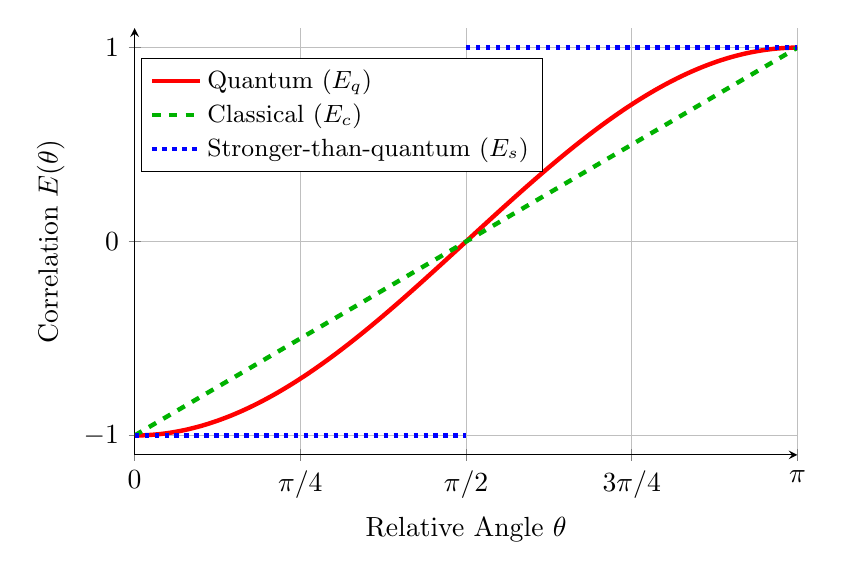
\begin{tikzpicture}
   \begin{axis}[
        xlabel={Relative Angle $\theta$},
        ylabel={Correlation $E(\theta)$},
        xmin=0, xmax=180, ymin=-1.1, ymax=1.1,
        axis lines=left,
        xtick={0, 45, 90, 135, 180},
        xticklabels={$0$, $\pi/4$, $\pi/2$, $3\pi/4$, $\pi$},
        ytick={-1, 0, 1},
        legend style={at={(0.01,0.93)}, anchor=north west, font=\small},
        legend cell align={left}, grid=major, width=10cm, height=7cm,
    ]
    \addplot[domain=0:180, samples=200, color=red, ultra thick] { -cos(x) };
    \addlegendentry{Quantum ($E_q$)}
    \addplot[domain=0:180, samples=2, color=green!70!black, dashed, ultra thick] { -1 + 2*x/180 };
    \addlegendentry{Classical ($E_c$)}
    \addplot[domain=0:90, samples=2, color=blue, dotted, ultra thick] { -1 };
    \addlegendentry{Stronger-than-quantum ($E_s$)}
    \addplot[domain=90:180, samples=2, color=blue, dotted, ultra thick, forget plot] { 1 };
    \end{axis}
\end{tikzpicture}
}
    \caption{A comparison of the three correlation functions $E(\theta)$. The quantum (solid red) and classical (dashed green) correlations only achieve perfect anti-correlation at $\theta=0$. The stronger-than-quantum correlation (dotted blue) is perfect for all angles except $\theta = \pi/2$.}
    \label{fig:correlations}
\end{figure}

\textit{Thermodynamic Value and Robustness}.---The thermodynamic value of these correlations is not given by their degree of nonlocality but by their mutual information. For any no-signaling distribution with uniform marginals, $I(A:E)$ depends only on $E(\theta)$:
\begin{equation}
I_\theta(A:E) = \ln 2 - h_2\left(\frac{1+E(\theta)}{2}\right),
\label{eq:Itheta}
\end{equation}
where $h_2(p)=-p\ln p-(1-p)\ln(1-p)$ is the binary entropy in nats. This relation follows from $I(A:E) = H(A) - H(A|E)$, where the marginal entropy is $H(A)=\ln 2$ and the conditional entropy $H(A|E)$ depends on the correlation's imperfection.

As shown in Fig.~\ref{fig:mutual_information}, perfect correlation or anti-correlation ($|E(\theta)|=1$) yields the maximal mutual information $I=\ln 2$. Consequently, according to Eq.~\eqref{eq:work_from_I}, the maximum work extractable per bipartite system is universally bounded by $k_{\mathrm{B}}T\ln 2$. This peak value is achievable in all three models, for instance, by aligning the measurement bases ($\theta=0$).

\begin{figure}[ht!]
\pgfmathdeclarefunction{h2}{1}{%
  \pgfmathparse{-((#1)==0 ? 0 : (#1)*ln(#1)) - ((1-#1)==0 ? 0 : (1-#1)*ln(1-#1))}%
}
\resizebox{0.4\textwidth}{!}{
    \begin{tikzpicture}
        \begin{axis}[
            xlabel={Relative Angle $\theta$},
            ylabel={Mutual Information $I(\theta)$ (nats)},
            xmin=0, xmax=180, ymin=-0.05, ymax=0.75,
            axis lines=left,
            xtick={0, 45, 90, 135, 180},
            xticklabels={$0$, $\pi/4$, $\pi/2$, $3\pi/4$, $\pi$},
            ytick={0, 0.6931}, yticklabels={0, $\ln 2$},
            legend style={at={(0.5, 0.75)}, anchor=center, font=\small},
            legend cell align={left}, grid=major, width=10cm, height=7cm,
        ]
        \addplot[domain=0:180, samples=201, color=red, ultra thick] { ln(2) - h2( (sin(x/2))^2 ) };
        \addlegendentry{Quantum ($I_q$)}
        \addplot[domain=0:180, samples=101, color=green!70!black, ultra thick, dashed] { ln(2) - h2(x/180) };
        \addlegendentry{Classical ($I_c$)}
        \addplot[domain=0:180, samples=2, color=blue, dotted, ultra thick] { ln(2) };
        \addlegendentry{Stronger-than-quantum ($I_s$)}
        \addplot[only marks, mark=*, mark size=3pt, color=blue, fill=white] coordinates {(90, {ln(2)})};
        \addplot[only marks, mark=*, mark size=2pt, color=blue, fill=blue] coordinates {(90, 0)};
        \end{axis}
    \end{tikzpicture}
}
    \caption{Mutual information versus measurement angle $\theta$. All models achieve the maximum value of $\ln 2$, but their robustness to misalignment differs. Classical information (dashed green) degrades linearly from the peak, while quantum (solid red) degrades quadratically, offering superior resilience.}
    \label{fig:mutual_information}
\end{figure}

This thermodynamic equivalence in peak yield belies a critical operational difference: robustness. The practical advantage of non-classical correlations becomes apparent when considering misalignment from the optimal setting ($\theta=0$).
For a small misalignment $\delta\theta$, the classical mutual information degrades linearly: $I_c(\delta\theta) \approx \ln 2 - \mathcal{O}(\delta\theta)$. This makes the resource \emph{brittle} with respect to experimental noise.
In contrast, the quantum correlation $E_q(\theta)=-\cos\theta$ is stationary at its peak. The mutual information near $\theta=0$ is approximately $I_q(\delta\theta) = \ln 2 - h_2(\sin^2(\delta\theta/2)) \approx \ln 2 - \mathcal{O}(\delta\theta^2)$. This quadratic decay makes the quantum resource significantly more \emph{robust} against small imperfections in establishing a shared reference frame.
The stronger-than-quantum model represents the ultimate in operational flexibility, providing the maximal resource for any $\theta \neq \pi/2$, making coordination of measurement settings almost entirely unnecessary.

This operational hierarchy can be quantified by an "energetic" CHSH parameter, $\mathcal{S}_W$, where the correlation $E$ in the standard CHSH expression is replaced by the work potential $W = k_{\mathrm{B}}T I(\theta)$. For the standard CHSH angles, this simplifies to $\mathcal{S}_W = k_{\mathrm{B}}T |3I(\pi/4) - I(3\pi/4)|$. Evaluating this for our three models reveals a strict hierarchy mirroring their robustness:
\begin{equation}
\mathcal{S}_W^{(c)} < \mathcal{S}_W^{(q)} < \mathcal{S}_W^{(s)}.
\end{equation}
Specifically, we find $\mathcal{S}_W^{(c)} \approx 0.25 k_{\mathrm{B}}T$, $\mathcal{S}_W^{(q)} \approx 0.54 k_{\mathrm{B}}T$, and $\mathcal{S}_W^{(s)} = 2 k_{\mathrm{B}}T \ln 2 \approx 1.39 k_{\mathrm{B}}T$. Stronger non-locality thus translates directly into a more valuable and resilient thermodynamic resource under the operational constraints of a Bell test.

\textit{Conclusion}.---Correlations between a system and its environment are a thermodynamic fuel, universally limited by their mutual information. A single perfectly correlated bit can yield at most $k_{\mathrm{B}}T\ln 2$ of work, as exemplified by a Szilard engine powered by shared information. The hierarchy among classical, quantum, and stronger-than-quantum correlations lies not in this peak value but in the robustness with which it can be accessed. Quantum correlations provide a distinct operational advantage over classical ones through their resilience to misalignment, a feature directly linked to their non-local character. Engines consuming correlations do not violate the second law; they demonstrate that information must be treated as a physical resource. Consequently, a truly isolated system must be sealed not only from exchanges of energy and matter, but also from preexisting informational ties to its surroundings.


\textbf{Author Contributions:} The author conceived and designed the study, performed the analysis, interpreted the results, and wrote the manuscript.

\textbf{Data availability statement:} Data sharing not applicable to this article as no datasets were generated or analysed during the current study,

\begin{acknowledgments}
This research was funded in whole or in part by the Austrian Science Fund (FWF) Grant DOI: 10.55776/PIN5424624. The author acknowledges TU Wien Bibliothek for financial support through its Open Access Funding Programme.
\end{acknowledgments}

\bibliography{svozil}

\end{document}
